% R1 independent reading of scan009. Literal irregular letters and unfinished statements retained.
\usetikzlibrary{calc}
\scanpage{9}\mspage{8}
J'explicite, à cause de son importance, la propriété suivante, bien qu'elle sera conséquence de diverses façons d'autres

% slanted
\margin{\tikz[x=.4em,y=.4em]{\draw (0,0)--(3.0,2.1);}\quad\uline{NB} La chose importante est $X'\mathrel{\tikz[baseline=-.4ex,x=.65em,y=.65em]{\draw (0,1.1)--(1,.5)--(0,-.1) (1,1.1)--(0,.5)--(1,-.1);}}Y'$, alors $X'\cap Y'=\varnothing$ immédiat. Car $Z\deleted{\ll}\leq X',\,Z\leq Y'$ $\Longrightarrow Z\ll X,\,\unsure{Z'|Z}\ll Y$ d'où $Z\ll X\cap Y=L$, or $Z\leq X'\parallel L\Longrightarrow Z\parallel L$, or $Z\ll L$ et $Z\parallel L$ \deleted{impossible} (\unsure{d'où|comme} $Z\mathrel{\tikz[baseline=-.4ex,x=.65em,y=.65em]{\draw (0,1.1)--(1,.5)--(0,-.1) (1,1.1)--(0,.5)--(1,-.1);}}L$) $\Longrightarrow Z\leq L$ \deleted{\unsure{absurde}} car \uline{$Z\cap L=\varnothing$ !}}%

% Two long diagonal cancellations and the open lower return stroke.
\figure{\begin{tikzpicture}
\node[anchor=north west,inner sep=0pt,text width=.93\linewidth,font=\small] (old) at (0,0) {%
\deleted{\uline{At} DC 1 : Soient $X,Y\in\unsure{M|\mathcal M}$ avec $X\deleted{\parallel}\mathrel{\tikz[baseline=-.4ex,x=.65em,y=.65em]{\draw (0,1.1)--(1,.5)--(0,-.1) (1,1.1)--(0,.5)--(1,-.1);}}Y\unsure{\text{\S}|?|.}$}
\deleted{\deleted{\unsure{Alors}} \inserted{Soient} $X'\ll X$, \deleted{$Y'\ll Y\Longrightarrow X'\parallel Y'$} \inserted{avec $X'\parallel X\cap Y=L$, (i.e. $X'\parallel Z$ pour $Z\leq X,Y$)} $Y'\ll Y$ avec $Y'\parallel L$. Alors $X'\parallel Y'$}



\deleted{\uline{Cor} 1 Soient $F,C\in\unsure{\mathscr F|\mathcal F}$ avec $F\parallel\unsure{C|G}$. Alors $F\ll F$, $C'\ll G\Longrightarrow F'\parallel G'$.}
\deleted{\uline{Cor. 2} Soient $F,G\in\mathscr F$, $F\mathrel{\tikz[baseline=-.4ex,x=.65em,y=.65em]{\draw (0,1.1)--(1,.5)--(0,-.1) (1,1.1)--(0,.5)--(1,-.1);}}G$ \deleted{$\unsure{L=\underset{Z\in\widetilde F\cap\widetilde G}{\mathrm{Sup}}\,Z}$} \inserted{$L=F\cap G$}, $F'\ll F,C'\ll G$. Supposons $F'\parallel L,\ G'\parallel L$, alors $F'\parallel G'$.}

\deleted{\uline{At DC} 2 \quad (Axiome des ateliers spacieux) \deleted{\unsure{Soit|Soient}} $X,Y\in M$, $\deleted{\unsure{L}}K=X\cap Y=\underset{Z\in\widetilde X\cap\widetilde Y}{\mathrm{Sup}}\,Z$. Supposons que pour tt $X',Y'$, avec $X'\ll X,\underline{Y'\ll Y,\ X'\parallel K},Y'\parallel K$, on ait $X'\parallel Y'$. Alors}
};
\draw ($(old.north west)!.02!(old.north east)+(0,.8em)$)--($(old.south west)!.50!(old.south east)+(0,.6em)$);
\draw ($(old.north west)!.56!(old.north east)+(0,.5em)$)--($(old.south west)!.93!(old.south east)+(0,4.0em)$);
\draw ($(old.south west)+(.2em,-.15em)$)..controls($(old.south west)+(6em,.2em)$)and($(old.south west)+(12em,.2em)$)..($(old.south west)+(18em,-.1em)$)--($(old.south west)+(24em,-.18em)$)..controls($(old.south west)+(24.5em,.6em)$)and($(old.south west)+(25em,2.2em)$)..($(old.south west)+(26.2em,2.7em)$);
\end{tikzpicture}}

On voudra la

\uline{Propriété 1} Soient $F,G\in\mathscr F$, $F\mathrel{\tikz[baseline=-.4ex,x=.65em,y=.65em]{\draw (0,1.1)--(1,.5)--(0,-.1) (1,1.1)--(0,.5)--(1,-.1);}}G$, $L=F\cap G$. Soient $F'\ll F,\ G'\ll G$. Alors
\[
\begin{aligned}
 & F'\mathrel{\tikz[baseline=-.4ex,x=.65em,y=.65em]{\draw (0,1.1)--(1,.5)--(0,-.1) (1,1.1)--(0,.5)--(1,-.1);}}G'\\
\Longleftrightarrow\quad & F'_{L}\mathrel{\tikz[baseline=-.4ex,x=.65em,y=.65em,line cap=round]{\draw (0,1.1)--(1,.5)--(0,-.1) (1,1.1)--(0,.5)--(1,-.1);\draw[line width=.95pt] (.14,.62)--(.85,.65)--(.13,.26)--(.9,.12) (.91,.96)--(.12,.34)--(.78,.31)--(.1,-.16);}}G'_{L}
\end{aligned}
\]

cf \deleted{p.} GF $\underline{\overline{\mathrm{VI}}}$, p.~\uline{\unsure{73|13}} -- On a en tous cas tjrs $\mathrel{\tikz[baseline=-.25ex,x=.55em,y=.45em,line cap=round]{\draw (0,.2)--(1.05,.2) (.1,.47)--(1.02,.47);\draw (1.12,.72)..controls(1.29,.58)and(1.36,.17)..(1.38,-.04)..controls(1.30,-.12)and(1.18,-.14)..(1.08,-.14);}}$
\deleted{\unsure{Montrons} qu'on a bien en $\Rightarrow$. En effet,}

Ceci est équivalent (si on le voit de façon générale) à l'ancien At 12, qui prend le nom

% slanted
\margin{\uline{Critère} de \uline{compatibilité} pour les raffinements de \uline{sous-figures}\quad Mais c'est faux dans le cas simplicial, ex :}%
\figure{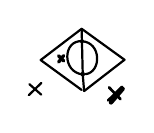
\begin{tikzpicture}[x=1em,y=1em,line cap=round,line join=round]
\draw[thick] (1.48,.04)--(0,1.12)--(1.48,2.25)--(3.03,1.13)--(1.57,0);
\draw[thick] (1.62,.61) .. controls (2.20,.68) and (2.20,1.76) .. (1.49,1.80)
 .. controls (.80,1.85) and (.76,.68) .. (1.52,.60);
\draw[thick] (1.48,2.25)--(1.52,.59)--(1.57,0);
\fill (1.49,1.80) circle (.074) (1.52,.61) circle (.085);
\draw[line width=1.2pt] (.65,1.05)--(.83,1.28) (.65,1.27)--(.83,1.09);
\draw[thick] (-.41,.25)--(.02,-.13) (-.43,-.15)--(.02,.29);
\draw[line width=1pt] (2.47,.13)--(2.88,-.29) (2.44,-.34)--(2.94,.15);\draw[line width=1.6pt] (2.54,-.41)--(2.96,.08);
\end{tikzpicture}}
% slanted
\margin{Mais on aura $X'_{L}\parallel Y'_{L}\Longrightarrow X'\mathrel{\tikz[x=.55em,y=.60em,line cap=round]{\draw (0,-.12)--(0,1) (.48,-.12)--(.48,1) (-.06,.30)--(.54,.47) (-.05,.51)--(.53,.65);}}Y'$, C'est un \unsure{contre-exemple|contre-exple|contre exemple} à l' \unsure{:|.} At $\parallel$, et a fortiori à \unsure{\deleted{ex}|ex} At 11 (cf GF $\underline{\overline{\mathrm{VI}}}$, p. 67,68)}%

\figure{\begin{tikzpicture}
\node[anchor=north west,inner sep=0pt,text width=.92\linewidth] (ax) at (0,0) {\uline{At DD} 1 \tikz[baseline=(so.base)]{\node[inner sep=0pt] (so) {Soient};\node[anchor=south west,rotate=43,inner sep=0pt] at (so.north east) {\inserted{ancien}};} $X,Y\ \mathrel{\tikz[baseline=-.3ex,x=.48em,y=.65em,line cap=round]{\draw (.4,.9)..controls(-.05,.8)and(-.08,.04)..(.35,.04)..controls(.66,.04)and(.6,.6)..(.3,.63);\draw (.43,.33)--(.66,.35) (.33,.03)--(.36,-.1);}}\ X',Y'\in M$, $X\mathrel{\tikz[baseline=-.4ex,x=.65em,y=.65em]{\draw (0,1.1)--(1,.5)--(0,-.1) (1,1.1)--(0,.5)--(1,-.1);}}Y,\ X'\ll X,Y'\ll Y$. Posons $K=X\cap Y=\underset{Z\in\widetilde X\cap\widetilde Y}{\mathrm{Sup}}\,Z$. Alors $X'_{L}\mathrel{\tikz[baseline=-.4ex,x=.65em,y=.65em]{\draw (0,1.1)--(1,.5)--(0,-.1) (1,1.1)--(0,.5)--(1,-.1);}}Y'_{L}$ implique $X'\mathrel{\tikz[baseline=-.4ex,x=.65em,y=.65em]{\draw (0,1.1)--(1,.5)--(0,-.1) (1,1.1)--(0,.5)--(1,-.1);}}Y'$ \quad (NB l'inverse\unsure{\, :|\, .|\,} \deleted{est} est tjrs vrai)};
\draw ([xshift=-.65em,yshift=-1em]ax.north west)--([xshift=-.65em,yshift=1em]ax.south west);
\end{tikzpicture}}

\uline{Corollaire} 1 \quad \unsure{la|le} ``propriété'' ci dessus

\[
F\parallel G,\ F'\ll F,\ G'\ll G\ \Longrightarrow\ F'\parallel G'
\tag*{\makebox[0pt][r]{\makebox[\displaywidth][l]{\uline{Corollaire} 2}}}
\]

Plus gén. \quad Si $F\mathrel{\tikz[baseline=-.4ex,x=.65em,y=.65em]{\draw (0,1.1)--(1,.5)--(0,-.1) (1,1.1)--(0,.5)--(1,-.1);}}G,\ F'\ll F,\ G'\ll G$, alors
\[
 F'\parallel G'\ \Longleftrightarrow\ F'_{L}\parallel G'_{L}
\]
